\documentclass[12pt]{article}
\usepackage[utf8]{inputenc}
\usepackage[english]{babel}
\usepackage{amsmath}
\usepackage[margin=1in]{geometry}
\usepackage{fancyhdr}
\pagestyle{fancy}
\lhead{DAFoam User Guides}
\rhead{}
\usepackage{biblatex}
\addbibresource{bibliography.bib}
\usepackage{multicol}
\usepackage{graphicx}
\usepackage{xurl}
\usepackage{hyperref}
\thispagestyle{empty}
\hypersetup{
    colorlinks=true,
    linkcolor=blue,
    filecolor=red,      
    urlcolor=blue,
    citecolor=blue,
}

\author{
Author: Janeita Reid\\
\linebreak
Reviewed by: Ping He\\
}

\date{\today}

\renewcommand*\contentsname{Contents}
\sloppy

\begin{document}
\title{Free-Form Deformation (FFD)}

  
\maketitle
  
\tableofcontents


\section{General Theoretical and Mathematical Preliminaries}

Before we explain how to setup the FFD points for the pyGeo\footnote{https://github.com/mdolab/pygeo} module from the \href{https://github.com/mdolab/MACH-Aero}{MACH-Aero framework}, it's essential to first understand underlying theoretical and mathematical formulations. In doing so, the user will gain a better understanding of pyGeo's strengths and weaknesses and how these influence constrained optimization in any of the disciplines supported by DAFoam (aerodynamics, solid mechanics and hydrodynamics). The guidelines covered in this section are for general applications using FFD. More specific guidelines  will be given in the sections that follow to highlight the features of the FFD module in MACH-Aero.\vspace{4mm} 

\begin{figure}[ht]
    \centering
    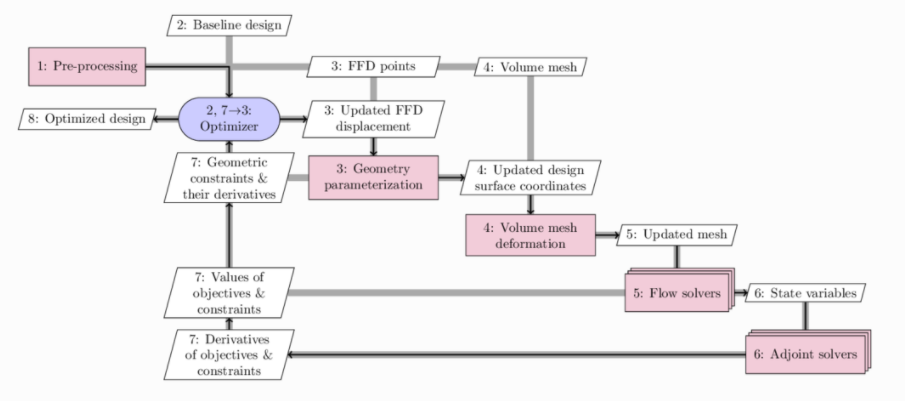
\includegraphics[width=1\textwidth]{pygeo.PNG}
    \caption{The pyGeo module for geometry parametrization (node 3) in the MACH-Aero framework \cite{machaero}}.
    \label{fig:my_label}
\end{figure}

\noindent pyGeo is closely tied to the concepts supporting free form deformation (FFD). FFD was first presented by Sederberg and Perry as a method for sculpting solid models by conducting global or local deformations \cite{sederberg}. The classic method involves a $R^3$ $\rightarrow$ $R^3$ mapping using trivariate tensor product Bernstein polynomials\cite{sederberg}, but this approach has evolved to also use  tri-variate Bézier, B-spline or NURBS volumes \cite{kenway} for mapping and remapping object points. The FFD approach adopted in pyGeo was developed by Kenway and Martins \cite{kenway}.\vspace{4mm} 

\noindent To get a better understanding of how FFD works, one can imagine putting an object or any geometry into a clear, flexible plastic-like shape that is transparent. In other words, by using FFD the geometry of the object is embedded into a volume that can be manipulated by moving points at the surface known as FFD points \cite{He2018}. \vspace{4mm} 


\noindent In order to manipulate the object and arrive at an optimized geometry, there are three steps involved in FFD, namely : 

\begin{enumerate}
    \item Create an initial FFD box with volumetric control points (aka. FFD points).
    \item Embed the design surface into the FFD box and find the mapping between the design surface's physical coordinates (x,y,z) and the FFD's parameter space (u,v,w).
    \item Deform the design surface by moving the FFD control points.
\end{enumerate}

\noindent To transform the steps above into mathematical formulations we take four things into consideration: the vertices of the initial embedded object given by $\overrightarrow{P}(u,v,w)$, the parametric space represented by $(u_0,v_0,w_0)$, control points (FFD points) on the initial deformation lattice given by $\overrightarrow{Q}_{i,j,k}$, and the vertices of the deformed object represented by $P^{new}(u_0,v_0,w_0)$ with new FFD points$\overrightarrow{Q}_{i,j,k}^{new}$ .\vspace{4mm} 

\noindent Additionally, basic knowledge of B-spline curves, surfaces or volumes presented by Kenway and Martins \cite{kenway} is also necessary to understand the parametrization of different objects.\vspace{4mm} 

For curves we have:
\begin{equation}
    C(u)=\sum_{i=0}^{N_{u}-1}N_{i,m_u}(u)Q_i
\end{equation}

For surfaces we have:\vspace{4mm} 
\begin{equation}
    S(u,v)= \sum^{N_{u}-1}_{i=0}\sum^{N_{v}-1}_{j=0}N_{i,m_u}(u)N_{j,m_v}(v)Q_{i,j}
\end{equation}

And for volumes we have: \vspace{4mm} 
\begin{equation}
    V(u,v,w)= \sum^{N_{u}-1}_{i=0}\sum^{N_{v}-1}_{j=0}\sum^{N_{w}-1}_{k=0} N_{i,m_u}(u)N_{j,m_v}(v)N_{k,m_w}(w) Q_{i,j,k}
\end{equation}

\noindent A good explanation of B-spline can be found here~\cite{Bspline}. With these in mind we develop the steps mentioned above considering the mathematical theory behind each of the three steps.\vspace{4mm} 

\textbf{Step 1}\\
The first step mentioned above represents the FFD module coupled with pyGeo. This tool will be elaborated further on in the tutorial. \vspace{4mm} 

\textbf{Step 2}\\
We need to consider that the embedded object which lies in a cartesian space is mapped into an initial trivariate B-spline volume using the equations below as given by Kenway and Martins \cite{kenway} and Ronzheimer \cite{Ronzheimer2004}. We have adopted the notations and overview presented by Ronzheimer \cite{Ronzheimer2002,Ronzheimer2004} with a small modification considering $Q_{i,j,k}^{new}$ instead of $R_{i,j,k}$. \vspace{4mm} 

\noindent For the mapping, a Newton method is used to calculate the parametric coordinates from given Cartesian coordinates\cite{Ronzheimer2006, He2018}. In other words, a mapping is determined between the FFD points (parameter space) and the surface geometry (physical space) \cite{He2018}. This is done by applying the Newton search on Equation 4 for each vertex of  $\overrightarrow{P}$ by solving for $u_0, v_0, w_0$ with the aim of mapping the points to the B-spline volume.

\begin{equation}
    \overrightarrow{P}(u,v,w)= \sum_{i=0}^{n_u}N_{i,m_{u}}(u),N_{j,m_{v}}(v),N_{k,m_{w}}(w)Q_{i,j,k}
\end{equation}

$N_{i,m_{u}}$, $N_{j,m_{v}}$ and $N_{k,m_{w}}$ are B-spline basis functions of degree $m_u$, $m_v$, and $m_w$. These are defined as knot vectors as follows:\vspace{4mm} 
\begin{enumerate}
    \item $N_i:{0,..,0,U_{m_{u+1}}...,U_{n_{u}},1,...,1}$
    \item $N_j:{0,..,0,v_{m_{v+1}}...,v_{n_{v}},1,...,1}$
    \item $N_k:{0,..,0,w_{m_{w+1}}...,w_{n_{w}},1,...,1}$
\end{enumerate}

The basis functions mentioned previously are calculated recursively using: 

\begin{equation}
   N_{i,1_{u}} = \begin{cases}
0, & u_i \le u <u_{i+1},\\
1, & \text{otherwise}. 
\end{cases}
\end{equation}
and
$$N_{i,m_{u}}(u) = \frac{u -u_i}{u_{i+m_{u-1}}-u_i}N_{i,m_{u-1}}(u) + \frac{u_{i+m_{u}}-u}{u_{i+m_{u}-u_{i+1}}}N_{i+1,m_{u-1}}(u)$$

\noindent \textbf{Step 3}\\
Finally, the B-spline volume that was calculated in Equation 4 is replaced by a new B-spline volume with control points $Q_{i,j,k}^{new}$. This is done by remapping the $u_0, v_0, w_0$ values previously calculated to obtain the deformed object point represented by $P^{new}(u_0,v_0,w_0)$. \vspace{4mm}

\begin{equation}
    \overrightarrow{P}^{new}(u_0,v_0,w_0)= \sum_{i=0}^{n_u}N_{i,m_{u}}(u_0),N_{j,m_{v}}(v_0),N_{k,m_{w}}(w_0)Q_{i,j,k}^{new}
\end{equation}

\noindent The initial control point lattice $\overrightarrow{Q}_{i,j,k}$ in Equation 4  and the new one in Equation 6 $Q_{i,j,k}^{new}$ perform the same function: to control the deformation of the embedded geometry. The final deformation of the embedded object is determined by $Q_{i,j,k}^{new}$. From Figure 2 it can be seen that the control lattice been deformed. This means that the initial points for $Q_{i,j,k}$ are no longer at their original position and have shifted creating a new control lattice $Q_{i,j,k}^{new}$. 

\begin{figure}[ht]
    \centering
    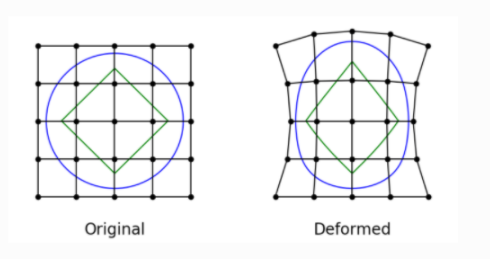
\includegraphics[width=0.75\textwidth]{deformedFFD.PNG}
    \caption{Before and after FFD points \cite{machaeroffd}}.
    \label{fig:my_label}
\end{figure}

\section{FFD considerations}
FFD is best suited for small to medium deformations \cite{Samareh2004} and proper constraints should be in place to ensure feasible geometry changes \cite{Anderson2012}. As a volumetric deformation method, FFD offers three advantages \cite{Anderson2012}: the embedded surface geometry has minimal effect on the computational cost, it is impartial to discrete geometry format, and the deformation quality is independent of the surface discretization quality. The main driver behind these advantages is that FFD volume parametrizes the \emph{geometry change} rather than the geometry itself \cite{kenway}; therefore, FFD eliminates the need for geometry abstraction and surface grid generation \cite{Samareh2004}. \vspace{4mm}

\noindent However, despite these advantages it's worth nothing that the grid topology is held fixed to ensure that as the design variables are modified, the function gradients are unaffected and remain continuous\cite{kenway}. The implication of this is that lattice controls the deformation of the object and there is no continuous interactive deformation involved. 

\section{FFD in DAFoam: pyGeo}
At the start of this tutorial, we noted that FFD allows the user to conduct both global and local deformation. Within pyGeo we can also control both the local and global shape of the geometry during optimization \cite{He2018}.The parametrization using pyGeo can be applied to structural domain, wetted surface of an aircraft \cite{kenway}, airfoil surface and wind turbine blade geometry.\vspace{4mm} 

\noindent In the example that follows, we will look at how to conduct a aerodynamic analysis of the NACA 0012 airfoil and the steps taken by pyGeo to parametrize the geometry. 

\subsubsection{Initial setup}
Before you configure the settings in your FFD folder its important to perform the following steps first: 
\begin{enumerate}
    \item Load your mesh in the appropriate folder. You can either use a mesh you generated from another program or run the meshing option configured in DAFoam. If you plan to use another mesh generated from another program, it won't be necessary to run the \textbf{preProcessing.sh} command to generate your mesh in DAFoam. You'll need to type blockMeshDict to populate your Polymesh file in the case folder if you use a grid generated from another program.
    \item Configure your runscript.py with the appropriate values for your particular case. For the case of optimizing for drag with lift constrained, you will need to first generate the correct angle of attack using the following command in your terminal: \textbf{mpirun -np 4 python runScript.py --task=solveCL}. But before you do that, continue to configure your runscript.py script until you reach the section \textbf{Design Variable Setup}. In the next sections we'll elaborate some more on what to do next. 
\end{enumerate}

\subsubsection{Point selection and Troubleshooting}

Within DAFoam you will be working with two files to modify your FFD points and control the geometric changes that are linked to the design variables in the adjoint equations: the Design Variable Setup section in the \textbf{runscript.py} and the \textbf{genFFD.py}.\vspace{4mm}


\begin{figure}[ht]
    \centering
    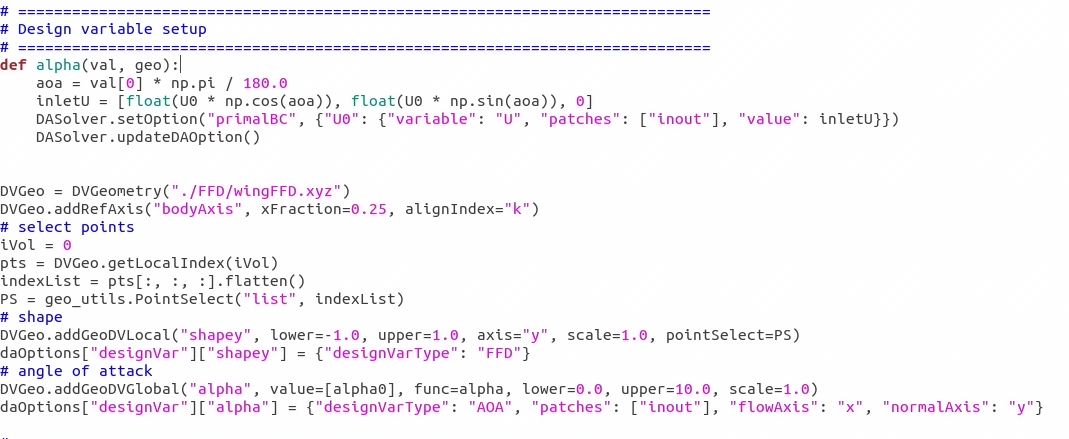
\includegraphics[width=1\textwidth]{FFDcodeshot.PNG}
    \caption{Code snippet from runscript.py highlighting the genFFD.py section credit: DAFoam}
    \label{fig:my_label}
\end{figure}

\noindent Before changing the parameters for the FFD points, assess your geometry to determine which parts of should be optimized and which should remain fixed. Parts of the geometry that will be optimized will be enclosed with FFD control point lattices. These points will then be manipulated according to the mathematical formulations explained above.\vspace{4mm}  

\noindent The number of FFD control points will influence the design freedom of an optimization problem. Hence, the number of FFD control points used does affect the fidelity of the final design: too few control points and we risk ignoring certain possibilities in the design space; too many design points and we could have issues with mesh overlap, an over crowded lattice and slower optimization. This is why it is important to choose the correct number of design points through trial and error and assess the final design to determine if the results reflect feasible applications.\vspace{4mm}  

\noindent The effect of the number of design control points was clearly seen in a study conducted by Ronzheimer \cite{Ronzheimer2006}. In the study it was shown that by doubling the number of FFD points from 4 to 8, the lift to drag ratio increased from 12\% to 16\% respectively. The optimization cycle also increased when the design points were doubled and clear differences in the final optimized shapes were noticed. Similar studies by Lyu, Kenway and Martins \cite{Lyu2014a} demonstrated that the effect of reducing the number of airfoil control points from 48 to 24 resulted in negligible effect on optimal shape and pressure while further decrease to 12 and then to 6 showed noticeable differences in drag and pressure coefficients.     \vspace{4mm} 

\noindent As a general guide we usually use 20 points for an airfoil section. However, users can use more or less depending on optimization goals. 

\subsubsection{Setting the Design Variables}

We set the design variable using the pyGeo module in the MACH-Aero framework by following the steps below in the \textbf{Design Variable Setup} section of the runscript.py script: 

\begin{enumerate}
\item Open the FFD folder in the case you are using for design optimization. It should look something like this below with the corresponding contents: 


\begin{figure}[ht]
    \centering
    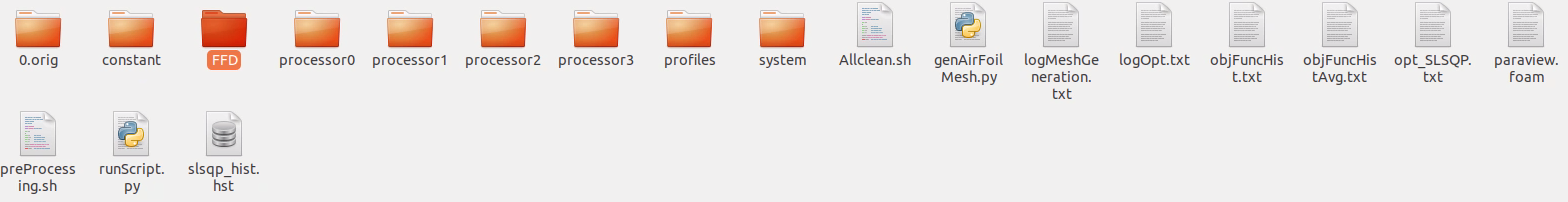
\includegraphics[width=0.85 \textwidth]{FFDcasefolder.PNG}
    \caption{ Typical case setup after running a simulation  credit:DAFoam}
    \label{fig:my_label}
\end{figure}

\begin{figure}[ht]
    \centering
    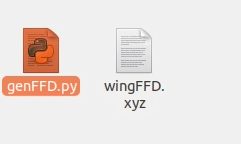
\includegraphics[width=0.55 \textwidth]{genFFd.PNG}
    \caption{FFD folder contents  credit: DAFoam}
    \label{fig:my_label}
\end{figure}

    \item Create a DVGeo object (DVGeo = DVGeometry(“./FFD/wingFFD.xyz”)) to manipulate the design surface geometry using the free-form deformation (FFD) approach. \textbf{NOTE: the FFD volume should completely contain the design surface}. The FFD file wingFFD.xyz is generated by running “python genFFD.py” in the FFD folder. We then add a reference axis (“addRefAxis”) for twist. Note that in this case we run 2D airfoil optimization, so no twist is needed, and “bodyAxis” is not used \cite{DAFoam}.
    
    There are two options to visualize the FFD points: 
    
    \begin{itemize}
        \item First copy the constant folder, the system folder, and paraview.foam to the FFD folder, then go to the FFD folder and run this command to convert the FFD mesh (plot3D format) to the OpenFoam mesh (plot3DToFoam -noBlank wingFFD.xyz) and use Paraview to load the FFD/paraview.foam file to view the FFD points.
    
        \item In version 2.2.1, we added a new utility to convert the plot3D file (*.xyz) format to the Tecplot format, such that you can load the FFD point in Paraview more easily (Paraview sometimes crashes when loading Plot3D files). To use it, just copy over the dafoam/dafoam/scripts/dafoam\_plot3d2tecplot.py file and run \texttt{python dafoam\_plot3d2tecplot.py wingFFD.xyz wingFFDTecplot.dat}. \textbf{NOTE: Be sure to copy dafoam\_plot3d2tecplot.py script to where you store the wingFFD.xyz file or else you will encounter problems}.

    \end{itemize}
    
    Now that you have done the necessary configurations in the genFFD.py file, the next step is to modify the runscript.py script at the Design variable setup mentioned earlier. 
    
    \item Once the FFD file is loaded and the reference axis is created, we select FFD points to move. The FFD file supports multi block meshes, but in this case we have only one block in the FFD, so we select “iVol = 0”. We allow all the points to move so we set “pts[:, :, :]” for “indexList”. Alternatively, we can select a subset of indices to move by setting a range for pts to move, e.g., indexList = pts[1:2, 3, 5:6].flatten() \cite{DAFoam}.
    
    
    \begin{figure}[ht]
    \centering
    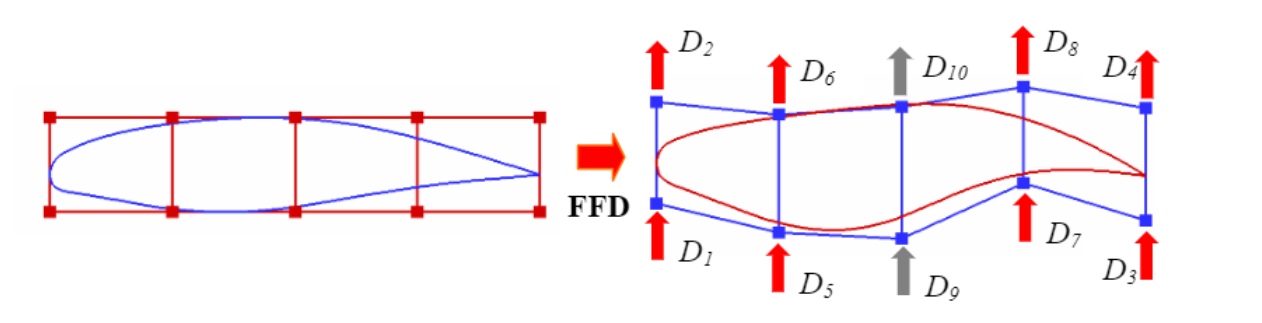
\includegraphics[width= 0.85 \textwidth]{FFDairfoil.PNG}
    \caption{Example with 8 FFD points where D9 and D10 are fixed \cite{Ronzheimer2004}}
    \label{fig:my_label}
\end{figure}
    
  \end{enumerate}  
  
\noindent If you intend to use one block to run your simulation then your block setup will look like this below.\vspace{4mm} 
    
    \begin{figure}[ht]
    \centering
    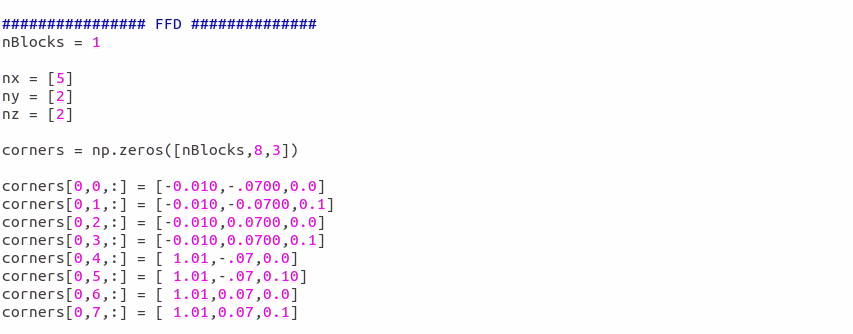
\includegraphics[width= 1 \textwidth]{FFDPY.PNG}
    \caption{FFD setup in genFFD.py}
    \label{fig:my_label}
\end{figure}

\noindent We'll notice that there is a nx, ny, nz. These mean the number of points in the x, y, z coordinates.\vspace{4mm}

\noindent For corners = np.zeros([nBlocks,8,3]):\vspace{4mm} 

\noindent The first entry is the FFD block number. In this case, there is only one block, that is why it is always zero. For examples using more than one blocks you can check the \href{https://dafoam.github.io/mydoc_tutorials_aero_dpw4.html}{DPW4} case or the \href{https://dafoam.github.io/mydoc_tutorials_aero_30n30p.html}{30N30P Multi-element airfoil} case where multiple FFD blocks are used, e.g., one for the wing and one for the tail.\vspace{4mm} 

\noindent The 2nd entry is the 8 corner indices, and the 3rd entry is the x,y,z coordinates of the corners.\vspace{4mm} 

\noindent If you intend to use two blocks then you'll need to modify the code to consider this type of configuration.
    
\subsubsection{Simulation Example: NACA 0012}

In this section we'll do a few examples to practice how to setup the getFFD.py and configure runscript.py. \vspace{4mm} 

\noindent \textbf{Step 1: Understand the Geometry You have}\\
\noindent Before we do any changes in the FFD files, we need to understand the type of geometry we are working with to know the limits of the FFD control points to consider. For a 2D airfoil such as NACA 0012 this means that were interested in the variations along the x and y axis. In this case we are using an airfoil with a blunt trailing edge where we removed a section. The coordinates the airfoil have been provided below for clarity. 

\begin{multicols}{2}
\noindent 0.0000000 0.0000000\\
 0.0005839 -.0042603\\
 0.0023342 -.0084289\\
 0.0052468 -.0125011\\
 0.0093149 -.0164706\\
 0.0145291 -.0203300\\
 0.0208771 -.0240706\\
 0.0283441 -.0276827\\
 0.0369127 -.0311559\\
 0.0465628 -.0344792\\
 0.0572720 -.0376414\\
 0.0690152 -.0406310\\
 0.0817649 -.0434371\\
 0.0954915 -.0460489\\
 0.1101628 -.0484567\\
 0.1257446 -.0506513\\
 0.1422005 -.0526251\\
 0.1594921 -.0543715\\
 0.1775789 -.0558856\\
 0.1964187 -.0571640\\
 0.2159676 -.0582048\\
 0.2361799 -.0590081\\
 0.2570083 -.0595755\\
 0.2784042 -.0599102\\
 0.3003177 -.0600172\\
 0.3226976 -.0599028\\
 0.3454915 -.0595747\\
 0.3686463 -.0590419\\
 0.3921079 -.0583145\\
 0.4158215 -.0574033\\
 0.4397317 -.0563200\\
 0.4637826 -.0550769\\
 0.4879181 -.0536866\\
 0.5120819 -.0521620\\
 0.5362174 -.0505161\\
 0.5602683 -.0487619\\
 0.5841786 -.0469124\\
 0.6078921 -.0449802\\
 0.6313537 -.0429778\\
 0.6545085 -.0409174\\
 0.6773025 -.0388109\\
 0.6996823 -.0366700\\
 0.7215958 -.0345058\\
 0.7429917 -.0323294\\
 0.7638202 -.0301515\\
 0.7840324 -.0279828\\
 0.8035813 -.0258337\\
 0.8224211 -.0237142\\
 0.8405079 -.0216347\\
 0.8577995 -.0196051\\
 0.8742554 -.0176353\\
 0.8898372 -.0157351\\
 0.9045085 -.0139143\\
 0.9182351 -.0121823\\
 0.9309849 -.0105485\\
 0.9427280 -.0090217\\
 0.9534372 -.0076108\\
 0.9630873 -.0063238\\
 0.9716559 -.0051685\\
 0.9791229 -.0041519\\
 0.9854709 -.0032804\\
 0.9906850 -.0025595\\
 0.9947532 -.0019938\\
 0.9976658 -.0015870\\
 0.9994161 -.0013419\\
 \end{multicols}

\noindent From the airfoil coordinates above, we see that your largest $x$ value is 0.9994161, while our largest $y$ value is 0.0600172. This means that the lattice/ block we create needs to be a bit bigger than 0.9994161 x 0.0600172. Let us choose one that is 1.01 x 0.07. It is important that the control lattice is body-fitted. If the lattice is too big for example 100 x 100 for the example above, then the gradient of dCD/dFFD will become very small (because the FFD point is far away from the design surface). The problem with this is that dCD/dFFD will have very different magnitudes compared with other design variables, say dCD/dAlpha with Alpha being the angle of attack. This will cause problems for the optimizer because it always wants to receive gradients with similar orders of magnitude. Hence, body-fitted FFD points should be used at all times. \vspace{4mm} 

\noindent \textbf{Step 2: Setup the FFD control points}

\noindent We know that we intend to use one block and that this one will have a dimension of 1.01 x 0.07. We now need to map out the points in this block. These points will represent the vertices of our control lattice. \vspace{4mm}

\noindent To create our FFD points we need to remember that NACA 0012 is a symmetric airfoil. We put our axis in the symmetric plane xy = 00 and start to map out our FFD control points.The order we choose to map out the control points is as follow: start with leading edge and then move to trailing edge. We have chosen to use 8 vertices for our block and will modify our genFFD.py to represent this.\vspace{4mm}  

\noindent The first point we enter is our coordinate with vertice (x,y) = (0,0). Although we have 2D airfoil, we are actually mapping out points for a 3D lattice as shown in the corners = np.zeros([nBlocks,8,3]). Taking this into consideration the point (0,0) will have coordinates $(-0.010,-.0700,0.0)$ on our lattice. This represents the leading edge control point in the negative y direction. The second point we consider is $(-0.010,-0.0700,0.1)$ which takes into consideration the thickness of our airfoil. Still at the leading edge we consider two more points to reflect the symmetry of our airfoil:[-0.010,0.0700,0.0] and [-0.010,0.0700,0.1]. The first point represents control point on the positive y direction, while the second point takes the thickness into consideration.\vspace{4mm} 

\noindent You will notice that so far only the leading edge and trailing edge points have been considered. This is because we need to prescribe the corners points for the FFD box, then the genFFD.py script will generate the coordinates for all other FFD points. To get a better understanding of this, check the \textbf{writeFFDFile} and \textbf{returnBlockPoints} functions in genFFD.py. \vspace{4mm}

\noindent \textbf{Step 3: Visualize the control points}

\noindent It's important that the control points cover the geometry, otherwise there will be errors. To visualize the control points, you can choose from two options as mentioned above. \vspace{4mm} 

\noindent \textbf{Step 4: Apply constraints}
 
\noindent Next we need to setup constraints to ensure that the optimized geometry is within feasible limits. To do this we use our runscript.py to modify the constraints. Here we can apply thickness constraints and volume constraints. FFD allows one to maintain constant volume even after geometry changes. \vspace{4mm}
 
\noindent Lower and upper projection points are used by the FFD during optimization to calculate the new thickness and volume change. An example of this is shown in the image below. More details can be obtained at \href{https://mdolab-mach-aero.readthedocs-hosted.com/en/latest/machAeroTutorials/opt_aero.html#geometric-constraints}{Mach Aero Tutorials}. \vspace{4mm}
 
 \begin{figure}[ht]
    \centering
    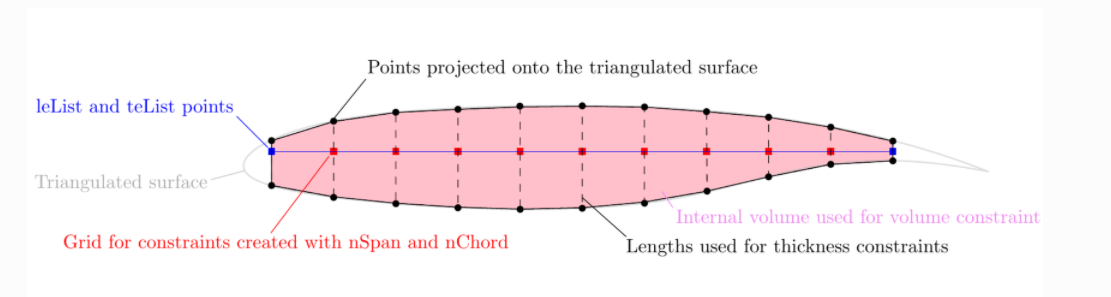
\includegraphics[width=1.0\textwidth]{thicknessconstraint.PNG}
    \caption{Example showing how volume and thickness constraints are calculated \cite{machaero2021}}.
    \label{fig:my_label}
\end{figure}
 
 
 \noindent \textbf{Step 5: Run simulation}
 
\noindent When all the necessary parameters are entered the next step is to run \textbf{mpirun -np 4 python runScript.py}. Check the result and move the control points if needed once the optimization is complete.

\section{Advanced Tips and Tricks}
\textbf{Ensure that your FFD points fully cover the design surface of your airfoil.} 
You can convert *.xyz file (FFD file) to the OpenFOAM format using this command: plot3dToFoam -noBlank wingFFD.xyz  Then you can load the FFD points and your OpenFOAM mesh into Paraview to check if FFD points fully contain the design surface.\vspace{4mm}

\section{Forum}
There is no better way to learn than to ask questions. You can post questions on the DAFoam \href{https://github.com/mdolab/dafoam/discussions}{forum} to get answers on bugs, general questions, tutorials, and installation. Before you post a question, first check out the best practices below:

\begin{enumerate}
    \item Check first to see if your question has already been answered.
    \item If your question has not been answered create a new discussion ensuring that: 
    \begin{itemize}
        \item The title of the question matches the details you'll provide.
        \item The most appropriate category has been selected for your question.
        \item Your question covers all the necessary details: what you did, what did not work, screenshots clearly showing details of your question, the results you were expecting and so on.
    \end{itemize}
\item If you find that you'll need to ask multiple questions on different topics, consider posting each topic separately as a new discussion. This way people are more likely to find the question instead of scrolling through a long thread. Of course, if keeping the discussion in one thread reduces the likelihood of confusion and makes it easier to follow how the problem gets solved then consider doing so.
\end{enumerate}
 \printbibliography
\end{document}